\documentclass[main.tex]{subfiles}
\begin{document}
\section{Commitment in $2\times2$ Games}\label{sec:GamePayoffs}
In the introduction, I presented a game in which commitment leads to strictly lower equilibrium payoffs. In this section I will investigate for which broader class of games this result holds. I analyze the effect of introducing commitment on equilibrium payoffs in a class of symmetric $2\times 2$ games. Specifically, I will consider $2\times2$ games that are symmetric in the sense of table \ref{tab:general2x2} (left) with $A<D$. To reduce the number of parameters without loss of generality, I apply a positive affine transformation: subtracting $A$ from all payoffs and dividing by $D - A$. This allows me to redefine the remaining parameters as $\bparam = \frac{B - A}{D - A}$ and $\cparam = \frac{C - A}{D - A}$, resulting in the normalized form shown in Table~\ref{tab:general2x2} (right). This transformation follows standard practice  \parencite[see][and references therein]{tewolde_game_2024}.
\begin{table}[h!]
\centering
\begin{tabular}{ccc}
    % First table
    \begin{tabular}{c|cc}
        & $A_1$ & $A_2$ \\[0.2em]
        \hline
        $A_1$ & $(A,A)$ & $(B,C)$ \\[0.2em]
        $A_2$ & $(C,B)$ & $(D,D)$ \\[0.2em]
    \end{tabular}
    &
    % Arrow
    \hspace{1em}
    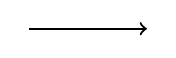
\begin{tikzpicture}[baseline=(current bounding box.center)]
        \draw[thick, ->] (0,0)--(1.5,0);
    \end{tikzpicture}
    \hspace{1em}
    &
    % Second table
    \begin{tabular}{c|cc}
        & $A_1$ & $A_2$ \\[0.2em]
        \hline
        $A_1$ & $(0,0)$ & $(\bparam,\cparam)$ \\[0.2em]
        $A_2$ & $(\cparam,\bparam)$ & $(1,1)$ \\[0.2em]
    \end{tabular}
\end{tabular}
\caption{Representation of a general $2\times 2$ game (left) and its simplified form (right).}
\label{tab:general2x2}
\end{table}
\subsection*{\centering Equilibria without Commitment}
Different values of $\bparam$ and $\cparam$ represent different types of well known $2\times2$ games. Figure \ref{fig:2x2-no-commitment} illustrates this.
\begin{figure}[h!]
    \centering
    \begin{tikzpicture}
        \begin{axis}[
            width=11cm,height=11cm,
            axis x line=middle,
            axis y line=middle,
            % Thicker, darker axes with clear arrow‑heads
            axis line style={ultra thick},
            xlabel={$\cparam$}, ylabel={$\bparam$},
            xmin=-1, xmax=2,
            ymin=-1, ymax=3,
            xtick={0,1},
            ytick={0,1},
            tick label style={font=\small},
            label style={font=\small},
            enlargelimits=false,
            clip=false
        ]
 
        % ---- lighter subdivision lines ---------------------------
        \addplot[black!70, thin] coordinates {(-1,1) (2,1)};   % horizontal at \bparam = 1
        \addplot[black!70, thin] coordinates {(1,1) (1,3)};    % vertical   at \cparam = 1
 
        % ---- striped grey fill for the top‑left region -----------
        \fill[pattern=north east lines, pattern color=gray!60]
             (axis cs:-1,1) -- (axis cs:0,1) -- (axis cs:0,3) -- (axis cs:-1,3) -- cycle;
        \fill[pattern=north east lines, pattern color=gray!60]
             (axis cs:2,1) -- (axis cs:0,1) -- (axis cs:0,-1) -- (axis cs:2,-1) -- cycle;
 
        % ---- region labels ---------------------------------------
        \node at (axis cs:-0.5, 0.5) {\large \textbf{Stag Hunt}};
        \node at (axis cs:-0.55,-0.5) {\large \textbf{Coordination}};
        \node[align=center] at (axis cs:1.5,2) {\large \textbf{Battle of}\\[2pt]\large \textbf{Sexes}};
        \node[align=center] at (axis cs:0.5,2) {\large \textbf{Game of}\\[2pt]\large \textbf{Chicken}};
 
        \end{axis}
    \end{tikzpicture}
    \caption{Game‑type regions in $(\cparam,\bparam)$‑space.}
    \label{fig:2x2-no-commitment}
\end{figure}
When $\bparam>1$ and $\cparam\in[0,1]$, the game takes the form of a Game of Chicken. Games with $\bparam>1$ and $\cparam>1$ are known as the Battle of Sexes. The Stag Hunt game arises when $\bparam \in [0, 1]$ and $\cparam < 0$. Finally, games with $\bparam < 0$ and $\cparam < 0$ do not really have a standard game name;  I refer to this residual class as Coordination games. Shaded areas denote games with strictly dominated strategies.
 
In pure strategies, the Game of Chicken and the Battle of Sexes have the Nash equilibria $\{A_1,A_2\}$ and $\{A_2,A_1\}$, whereas Stag Hunt and Coordination have the equilibria $\{A_1,A_1\}$ and $\{A_2,A_2\}$. All of these games have one equilibrium that involves mixing: Players play $A_1$ with probability $\frac{\bparam-1}{\cparam+\bparam-1}$, which yields the expected payoff $\frac{\bparam\cparam}{\bparam+\cparam-1}$. \footnote{The general game does not have a mixed equilibrium when $b+c=1$, in which case there are (weakly) dominated strategies.} Note that this MSNE is the unique symmetric equilibrium for the Game of Chicken and the Battle of Sexes.

\subsection*{\centering  Equilibria with Commitment}
Base game equilibria in pure strategies translate into subgame perfect Nash equilibria in pure strategies in the commitment game. This can occur in three distinct ways: both players committing upfront to base game equilibrium strategies, one player committing first and the other waiting and then best responding, or both players waiting and then subsequently playing equilibrium strategies. In the appendix in section~\ref{sec:proof1}, I establish two lemmas characterizing the conditions under which each type of pure strategy equilibrium arises. 
 
However, I argue that focusing on subgame perfect equilibria in \textit{mixed strategies} rather than pure strategies is considerably more compelling for two reasons: symmetry and equilibrium selection.
\paragraph{Symmetry} All $2\times2$ games considered in this section are symmetric, yet the Game of Chicken and the Battle of Sexes do not have a symmetric equilibrium in pure strategies, neither in the base game nor in the commitment version. Asymmetric equilibria seem counterintuitive. Players are identical in both strategy sets and payoffs, thus there is no clear rationale for why one should expect opposite equilibrium behavior. As I show, the mixed equilibrium is the unique symmetric equilibrium in these games, and thus seems better fitted as a solution concept to predict the behavior of players.
 
\paragraph{Equilibrium Selection} In each commitment game, multiple pure strategy Nash equilibria typically exist. Given the absence of communication devices and the one-shot nature of commitment games, it seems implausible that players can seamlessly coordinate on a single equilibrium. This is particularly relevant in the Game of Chicken and the Battle of Sexes, where each player prefers a different equilibrium. A mixed equilibrium naturally incorporates the possibility of miscoordination, quantifies the probability with which miscoordination might occur, and provides expected payoffs rather than deterministic outcomes. Additionally, Harsanyi’s purification theorem \parencite[]{harsanyi_games_1973} further supports the practical relevance of mixed equilibria. 
\begin{proposition}\label{theo:GamePayoffs}
Consider a symmetric $2\times2$ game and its commitment variant. In the unique mixed subgame perfect equilibrium of the commitment game, the expected payoff for both players relative to the mixed equilibrium of the base game is:
\begin{enumerate}
    \item weakly lower in the Game of Chicken (strictly for $\cparam<1)$;
    \item higher in the Battle of Sexes.
\end{enumerate}
\end{proposition}
\noindent Notably, Proposition~\ref{theo:GamePayoffs} establishes that commitment can induce equilibria in which both players are strictly worse off. To my knowledge, this finding is not documented in the existing literature. The proof is presented in the appendix in section \ref{sec:prooftheo1}, where the equilibria for all game-type regions are derived. 
 
Proposition \ref{theo:GamePayoffs} illustrates that the impact of commitment on player payoffs depends on the underlying game. In the Game of Chicken, commitment makes players worse off; in contrast, it improves outcomes in the Battle of the Sexes. 
To see why, consider the Game of Chicken with commitment. Committing to $A_2$ (moving out of the way) is weakly dominated by waiting, so players effectively choose between committing $A_1$ and $W$. 
The resulting reduced normal form is shown in Table \ref{tab:prop1-intuition}, which closely resembles the generalized $2\times2$ base game in Table~\ref{tab:general2x2}, except that $A_2$ is replaced by $W$, and the $(A_2,A_2)$ payoff is substituted by the “Wait–Wait payoff.”
In the base game, if both players play the non-aggressive strategy $A_2$, they receive the safe payoff $1$. However in the commitment game, if both play the non-aggressive strategy $W$, they receive the expected mixed equilibrium payoff of the base game, $\frac{\bparam\cparam}{\cparam+\bparam-1}$. This payoff is less than 1 in the Game of Chicken, where $b>1$ and $c\in(0,1]$. As a result, commitment transforms the Game of Chicken into one with worse outcomes. 
In the Battle of the Sexes, this dynamic is reversed. Since $b>1$ and $c>1$, the Wait-Wait payoff $\frac{\bparam\cparam}{\cparam+\bparam-1}$ exceeds 1, so commitment improves payoffs relative to the base game. 
%\textcolor{orange}{Additionally, $A_2$ is not weakly dominated, so players mix over $A_1$,$A_2$ and $W$, and thus further reduce the probability of miscoordination.}
\begin{table}[h!]
\centering
\begin{tabular}{ccc}
    % Modified table without A_2
    \begin{tabular}{c|cc}
        & $A_1$ & $W$\\[0.2em]
        \hline
        $A_1$ & $0,0$ & $\bparam,\cparam$\\[0.2em]
        $W$   & $\cparam,\bparam$ & $\tfrac{\bparam\cparam}{\cparam+\bparam-1},\tfrac{\bparam\cparam}{\cparam+\bparam-1}$\\[0.2em]
    \end{tabular}
\end{tabular}
\caption{Reduced Normal Form of the Game of Chicken with Commitment}
\label{tab:prop1-intuition}
\end{table}
\newline
While initially stated that all symmetric $2\times2$ games would be considered, Proposition~\ref{theo:GamePayoffs} focuses only on the Game of Chicken and the Battle of the Sexes. Corollary~\ref{cor:staghunt-coord}, derived in Appendix~\ref{sec:prooftheo1}, extends the analysis to the Stag Hunt and Coordination Game.
\begin{corollary}
    The following results hold for the Coordination Game and the Stag Hunt.

    \begin{enumerate}
        \item There is a mixed subgame perfect equilibrium in the Coordination Game. However, players committing to $(A_1,A_1)$ is another symmetric subgame perfect equilibrium that Pareto-dominates the mixed equilibrium.
        \item The Stag Hunt game does not have a mixed equilibrium.
    \end{enumerate}
    \label{cor:staghunt-coord}
\end{corollary}

\noindent Although Corollary \ref{cor:staghunt-coord} is instructive, the more interesting strategic dynamics arise in games such as the Game of Chicken and the Battle of the Sexes. Thus, in the next section, I will focus on these two game types.
\end{document}
